%%%%%%%%%%%%%%%%%%%%%%%%%%%%%%%%%%%%%%%%%%%%%%%%%%%%%%%%%%%%%%%%%%%%%%
% LaTeX Template: Two Column Colour Article
%
% Source: http://www.howtotex.com/
% Feel free to distribute this template, but please keep the
% referal to howtotex.com.
% Date: Feb 2011
% 
%%%%%%%%%%%%%%%%%%%%%%%%%%%%%%%%%%%%%%%%%%%%%%%%%%%%%%%%%%%%%%%%%%%%%%
% How to use overleaf.com: 
%
% You edit the source code here on the left, and the preview on the
% right shows you the result within a few seconds.
%
% You can upload figures, bibliographies, custom classes and
% styles using the files menu.
%
% If you're new to LaTeX, the wikibook is a great place to start:
% http://en.wikibooks.org/wiki/LaTeX
%
%%%%%%%%%%%%%%%%%%%%%%%%%%%%%%%%%%%%%%%%%%%%%%%%%%%%%%%%%%%%%%%%%%%%%%
% adaptions made by wolfgang stoettner mail@stoettner.net
%%%%%%%%%%%%%%%%%%%%%%%%%%%%%%%%%%%%%%%%%%%%%%%%%%%%%%%%%%%%%%%%%%%%%%

%%% Preamble
\documentclass[	DIV=calc,%
							paper=a4,%
							fontsize=11pt,%
							twocolumn]{scrartcl} % KOMA-article class
\usepackage[french]{babel}	% English language/hyphenation
\usepackage[protrusion=true,expansion=true]{microtype}	% Better typography
\usepackage{amsmath,amsfonts,amsthm} % Math packages
\usepackage{pythontex} % Math packages
\usepackage[pdftex]{graphicx} % Enable pdflatex
\usepackage{wrapfig} % enable figure wrapping
\usepackage[svgnames]{xcolor} % Enabling colors by their 'svgnames'
\usepackage[hang, small,labelfont=bf,up,textfont=it,up]{caption} % Custom captions under/above floats
\usepackage{epstopdf} % Converts .eps to .pdf
\usepackage{subfig}	% Subfigures
\usepackage{booktabs} % Nicer tables
\usepackage{fix-cm}	% Custom fontsizes
\usepackage{booktabs} % prof. looking tables (www.en.wikibooks.org/wiki/LaTeX/Tables#Professional_tables)
\usepackage{float}
\usepackage{tgtermes}
\usepackage[T1]{fontenc}
\usepackage[utf8]{inputenc}


%%% Custom sectioning (sectsty package)
\usepackage{sectsty} % Custom sectioning (see below)
\allsectionsfont{%		% Change font of al section commands
	\usefont{OT1}{phv}{b}{n}%	% bch-b-n: CharterBT-Bold font
	}

\sectionfont{%		% Change font of \section command
	\usefont{OT1}{phv}{b}{n}%	% bch-b-n: CharterBT-Bold font
	}
%%% Headers and footers
\usepackage{fancyhdr} % Needed to define custom headers/footers
	\pagestyle{fancy} % Enabling the custom headers/footers
\usepackage{lastpage}	

% Header (empty)
\lhead{}
\chead{}
\rhead{\today}
% Footer (you may change this to your own needs)
\lfoot{\footnotesize \texttt{formulaire capteur} \textbullet Antonin Kenzi}
\cfoot{}
\rfoot{\footnotesize page \thepage\ of \pageref{LastPage}}	% "Page 1 of 2"
\renewcommand{\headrulewidth}{0.0pt}
\renewcommand{\footrulewidth}{0.4pt}
\newcommand{\hformbar}[1]{\vspace{2pt}\hrule\vspace{5pt}} % creates a horizontal bar to separate formulae better; space adaptions can be made centrally here


%%% Creating an initial of the very first character of the content
\usepackage{lettrine}
\newcommand{\initial}[1]{%
     \lettrine[lines=3,lhang=0.3,nindent=0em]{
     				\color{DarkGoldenrod}
     				{\textsf{#1}}}{}}

%%% Title, author and date metadata
\usepackage{titling} % For custom titles

\newcommand{\HorRule}{\color{DarkGoldenrod}%	% Creating a horizontal rule
									  	\rule{\linewidth}{1pt}%
										}

\pretitle{\vspace{-30pt} \begin{flushleft} \HorRule 
				\fontsize{30}{30} \usefont{OT1}{phv}{b}{n} \color{DarkRed} \selectfont 
				}
\title{Formulaire Capteur} % Title of your article goes here
\posttitle{\par\end{flushleft}\vskip 0.1cm}

\preauthor{\begin{flushleft}\large \lineskip 0.1cm \usefont{OT1}{phv}{b}{sl} \color{DarkRed}}
\author{Kenzi Antonin}	% Author name goes here
\postauthor{\footnotesize \usefont{OT1}{phv}{m}{sl} \color{Black} \hspace{1pt}  \par\end{flushleft}\HorRule}
\date{\today} % No date

%%% wws: create a non-indented formula name
\newcommand{\formdesc}[1]{\noindent\textbf{#1}}

%%% Begin document -----------------------------------------------------------------
\begin{document}
\maketitle
\thispagestyle{fancy} 	% Enabling the custom headers/footers for the first page 
% The first character should be within \initial{}

\hformbar

\formdesc{Classification des mesurandes}
\begin{equation}
\label{Classification des mesurandes}
\end{equation}
\footnotesize il existe plusieurs catégories de mesurandes : 
\begin{enumerate}
 \item Mécanique : déplacement, vitesse... 
 \item Électrique : courant, tension, charge
 \item Thermique : température flux thermique
 \item Magnétique : champ magnétique, perméabilité
 \item Radiation : lumière visible, rayon X, radiation
 \item Bio/chimique :  humidité, gaz, sucre, hormones 
\end{enumerate}

\hformbar

\formdesc{Capteur et chaînes d'acquisition}
\begin{equation}
    \label{Capteur et chaînes d'aquisition}
\end{equation}
\begin{figure}[H]
    \begin{center}
        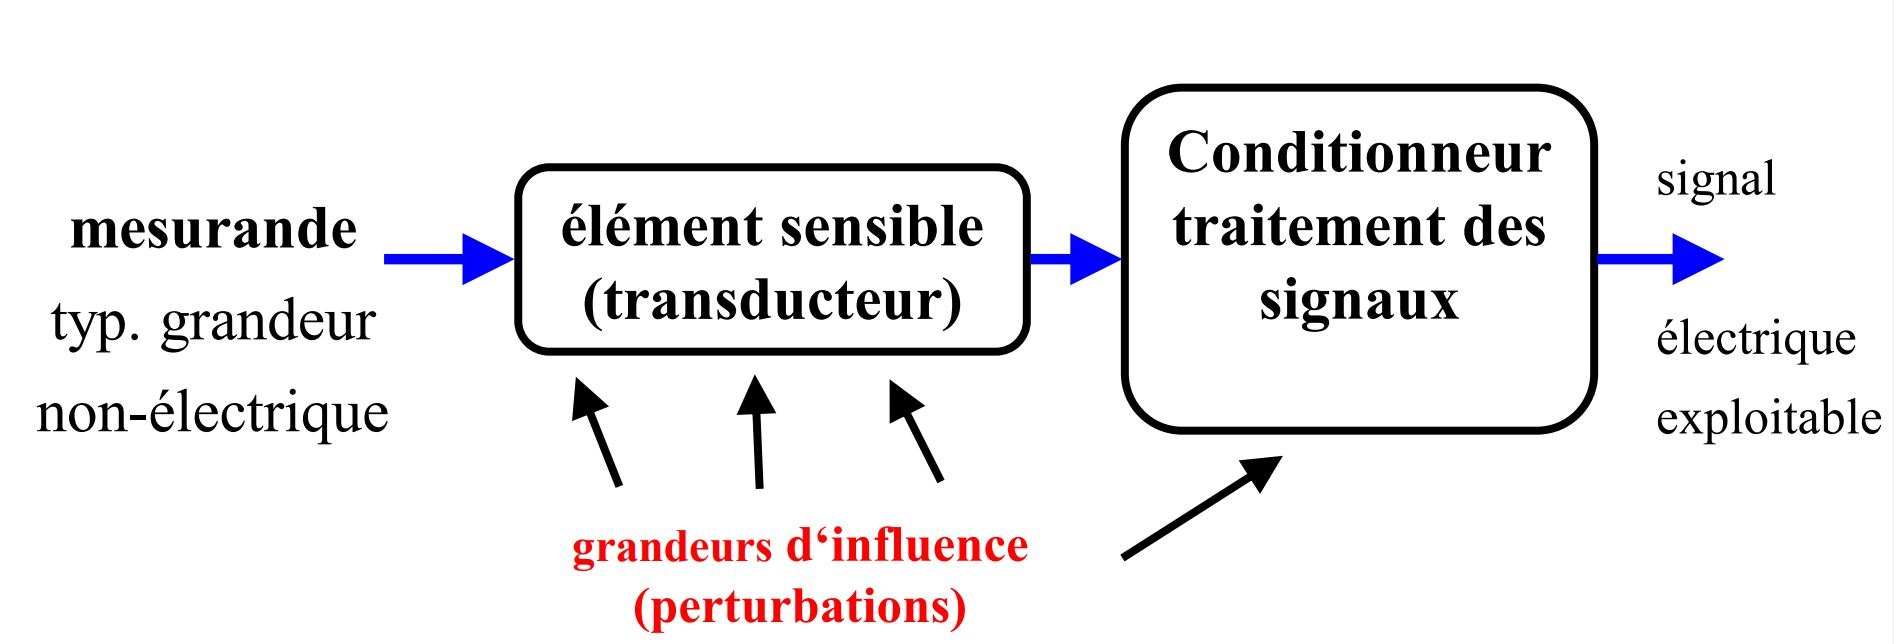
\includegraphics[width=0.3\textwidth]{img/capteur_influence.JPG}
        \caption{Illustration des influences}
        \label{fig:Illustration des influence}
    \end{center}
\end{figure}
Problèmes :
\begin{itemize}
 \item modifié par des grandeurs d'influence
 \item retard sur le signal
 \item un organe de mesure modifie l'environnement
\end{itemize}

\hformbar

\formdesc{Sensibilité du capteur}
\begin{equation}
    S = \cfrac{\Delta s}{\Delta m} \big |_mi
    \label{Capteur et chaînes d'aquisition}
    \end{equation}
\begin{figure}[H]
    \begin{center}
        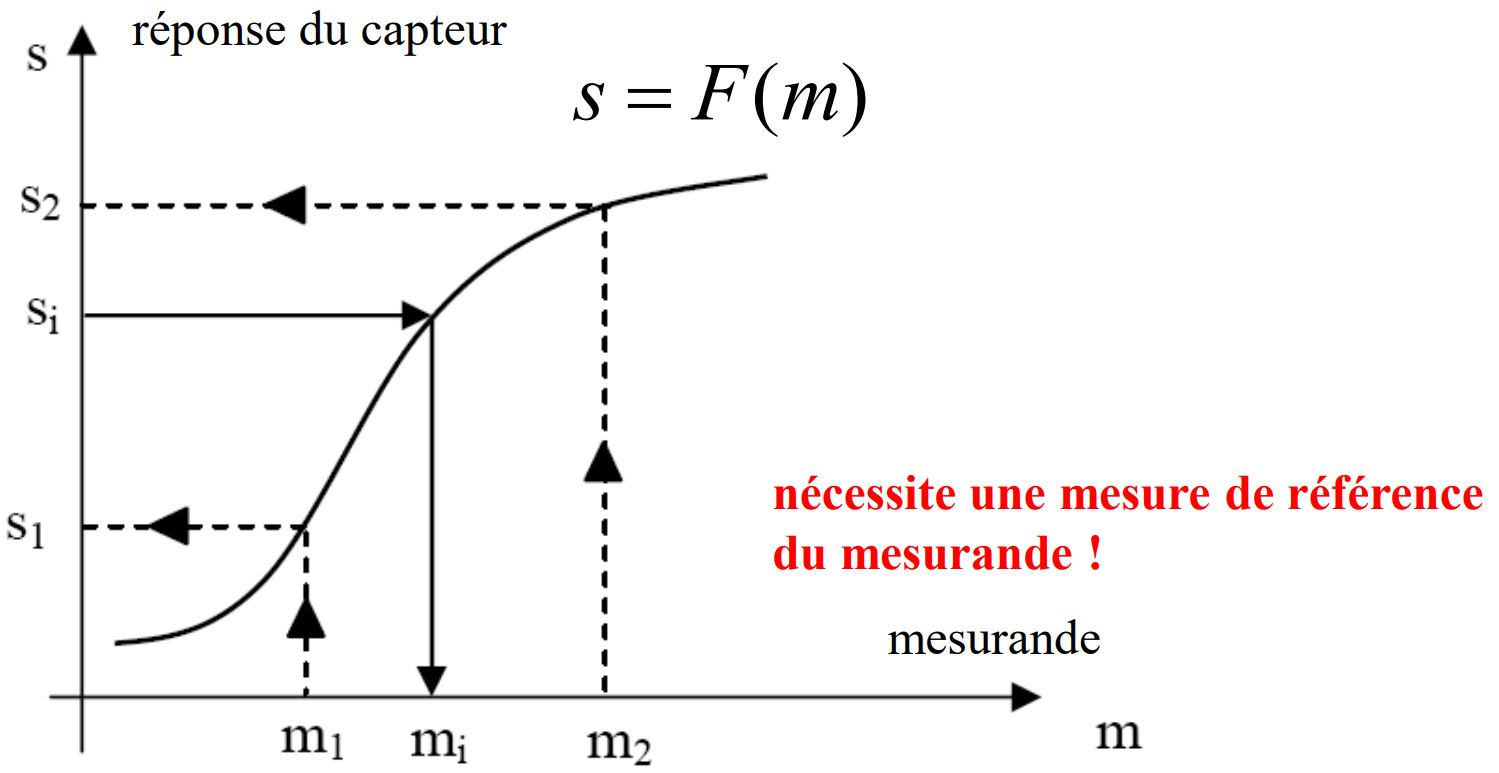
\includegraphics[width=0.3\textwidth]{img/Etalonage_statique.JPG}
        \caption{Etalonage Statique, Cas idéale}
        \label{fig:Etalonage Statique, Cas idéale}
    \end{center}
\end{figure}


\hformbar
\formdesc{Erreur de linéarité}
\begin{equation}
    \label{Capteur et chaînes d'aquisition}
    \end{equation}
\begin{figure}[H]
    \begin{center}
        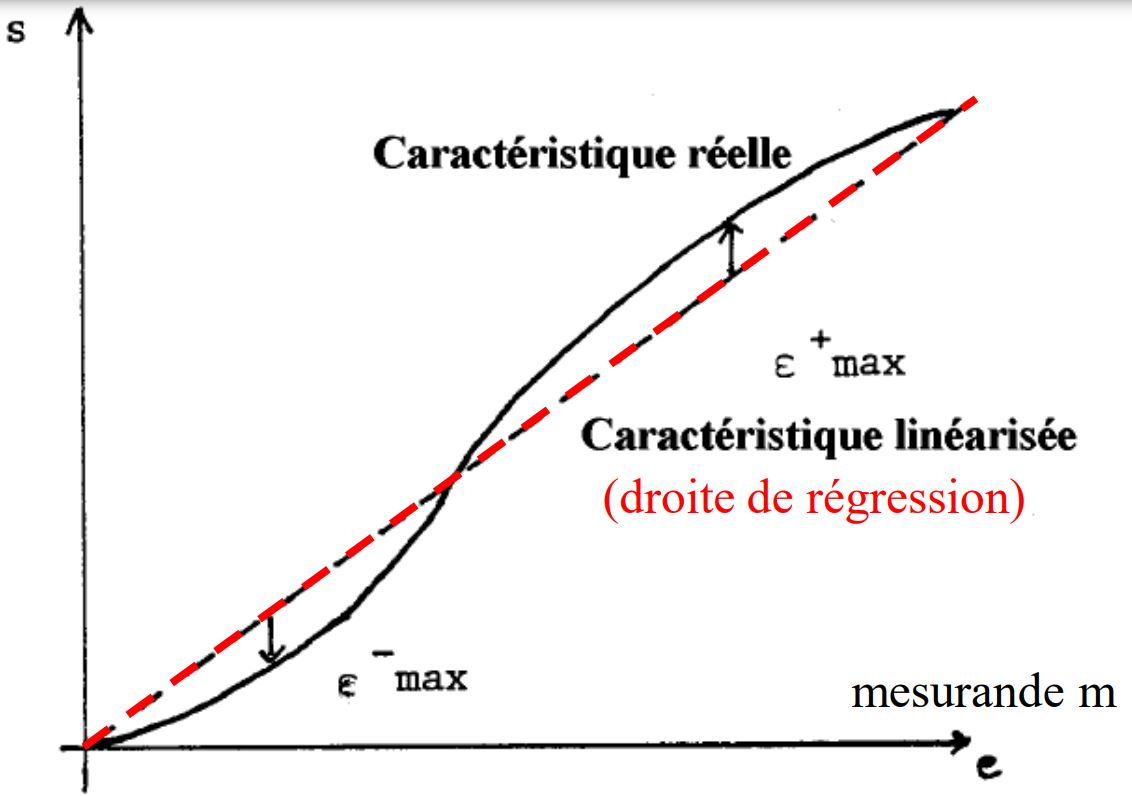
\includegraphics[width=0.3\textwidth]{img/linearite.JPG}
        \caption{Erreur de linéarité}
        \label{fig:Erreur de linéarité}
    \end{center}
\end{figure}
Elle s'exprime en \%, soit l'erreur relative maximale entre la droite de régression et la caractéristique réelle.

\end{document}